\subsection{Artificial neural network\label{s:ann}}

We tried to use artificial neural networks as a quick and somewhat accurate prediction of the outcome of a game a while before it ends by first training it on a labelled set of partially-completed games. The label indicates whether or not the current player will win (1), tie (0) or lose (-1). We always split our data set into a training and validation set using a 4:1 ratio. We also always used one hidden layer with as many neurons as the mean of the amount of neurons in the input and output layer (just one). As the activation function, we used the hyperbolic tangent. On a final note: we are aware that the two graphs presented in this section have a lower validation error than training error. Although this is strange, as far as we know it doesn't necessarily indicate a problem with the machine learning model.

\subsubsection{First approach}

First, we generated the games by letting two agents play random legal moves against each other, unless there are optimal moves (which are then played first), until at least 70\% of the edges have been filled and there are no optimal moves left. The feature vector used to represent the board to the ANN consisted of the current player's score, the other player's score and the number of open chains and loops of different lengths (chains of a length above the maximum are simply capped to that maximum in the feature vector). We don't consider half-open chains and closed chains since their presence implies the presence of optimal moves, which can be used first in MCTS before relying on a heuristic. Here are the results from a data set of 5000 games:

\begin{center}
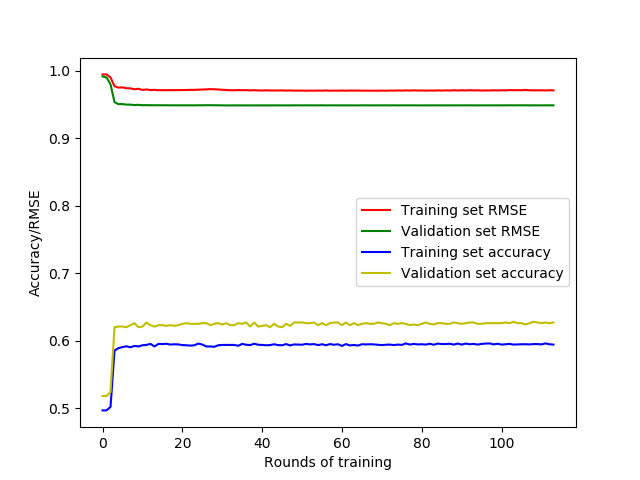
\includegraphics[scale=0.65]{images/ann_rmse+accuracy_(5000_games).png}
\end{center}

This ANN has an accuracy of 62.6\% on the validation set and 59.4\% on the training set, which isn't very high. In fact, after analyzing the weights it turns out the ANN is doing little more than just making a guess based on the difference in scores. This heuristic wasn't very satisfactory to us.

\subsubsection{More realistic boards and chain parity}

In our second approach, we actually let two semi-intelligent agents (namely, agent 4 from section 3.1) play against each other to create more realistic board scenarios. The simulation was halted at the point where the game reaches the state MIDDLE, as described in section 2.1.2. Our main idea is that during MCTS, any node in middle-game is evaluated using this heuristic, which provides a better estimate for the desirability of moves during early game. In end-game, the heuristic won't be used anymore but this is fine since MCTS with the aforementioned improvements should be able to play fairly well at this point (it's just end-game, after all).

	Secondly, we tried to incorporate a more advanced piece of "Dots and boxes" strategy into our agent, namely the "chain rule" [REFERENCE TO \url{http://web.archive.org/web/20070627082933fw_/http://cf.geocities.com/ilanpi/math.html#proof}]. This rule states that, in order to force the opponent to open up the first chain in end-game (which usually decides the game), the first player should aim to have the parity of the number of open chains of length larger than two equal the parity of dots on the board (it's the opposite for the second player). As such, we added a value to our feature vector which is 1 if the current chain parity is beneficial to the current player or -1 if it isn't. In games marked with the state MIDDLE, the exact number of chains isn't entirely decided yet, so the chain rules can't be simply applied to the current chain parity. Therefore, we tried to let our ANN learn a model which gives us non-trivial accuracy. Here are the results from a data set of 1000 games:
	
\begin{center}
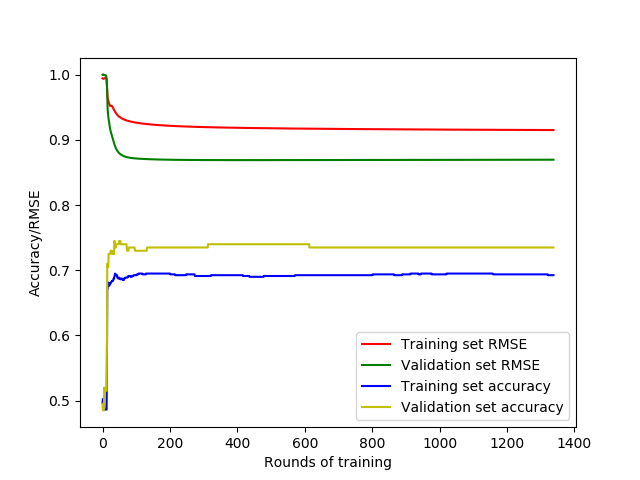
\includegraphics[scale=0.65]{images/ann_rmse+accuracy_(MCTS2_1000_games).png}
\end{center}

This gives us an accuracy of 73.5\% on the validation set and 69.25\% on the training set, which is a lot higher than the accuracy of the chain parity value on its own (51.1\%), which is why we decided to put this ANN into our agent.
